\chapter{Zprovoznění jednotlivých komponent}
\label{Zprovoznění jednotlivých komponent}
Jednotlivé komponenty jsou připojeny k mikrokontroléru podle obrázku č. \ref{blokove_schema}. Displej a klávesnici stačí jen připojit, proto je nebudu v rámci této kapitoly více rozebírat.

\section{Ověření přesnosti váhy}

Před použitím samotné váhy jsem ověřil, zda její přesnost odpovídá parametrům stanoveným výrobcem z důvodu, že váha není certifikovaná. Ověření probíhá pomocí druhé váhy nebo kalibrovaného závaží o jednu třídy přesnosti výše. Pro váhu integrovanou do měřícího systému G\&G E3000 je třída přesnosti III, proto je nutné volit váhu s třídou přesnosti II dle normy OIML R 76 nebo kalibrované závaží s třídou přesnosti M1 dle normy OIML R 111. Pro ověření přesnosti byla použita váha Kern PCB-2500-2 s padesátkrát vyšší přesností: 0,01 g a váživostí 2,5 kg. Obě váhy byly před použitím kalibrovány a použity v laboratorním prostředí s teplotou 20,4 °C a vlhkostí 28,7 \%, které odpovídají požadavkům obou výrobců vah pro přesná měření. Z tabulky č. \ref{tab:vahy} je vidět, že váha G\&G-3000 měří s požadovanou přesností 0,5 g. %a spadá tak do třídy přesnosti III.




%\begin{table}
%    \centering
%    \begin{tabular}{|c|c|}
%    \hline
%         \begin{tabular}[c]{@{}c@{}} Kern PCB-2500-2 \\ (g) \end{tabular} & \begin{tabular}[c]{@{}c@{}} G\&G E3000 \\ (g) \end{tabular}\\ \hline
%         20,00 & 20,0\\ \hline
%         200,00&200,0 \\ \hline
%         400,00&400,0 \\ \hline
%         600,00 & 600,0 \\ \hline
%         800,00&800,0 \\ \hline
%         1000,00&1000,0 \\ \hline
%         1200,00&1200,0 \\ \hline
%         1400,00&1400,0 \\ \hline
%         1600,00&1600,0 \\ \hline
%         1800,00&1800,0 \\ \hline
%         2000,00&2000,0 \\ \hline
%         2200,00&2200,0 \\ \hline
%    \end{tabular}
%    \caption{Ověření přesnosti váhy G\&G E3000}
%    \label{tab:vahy}
%\end{table}

\begin{figure}[H]
    \begin{center}
        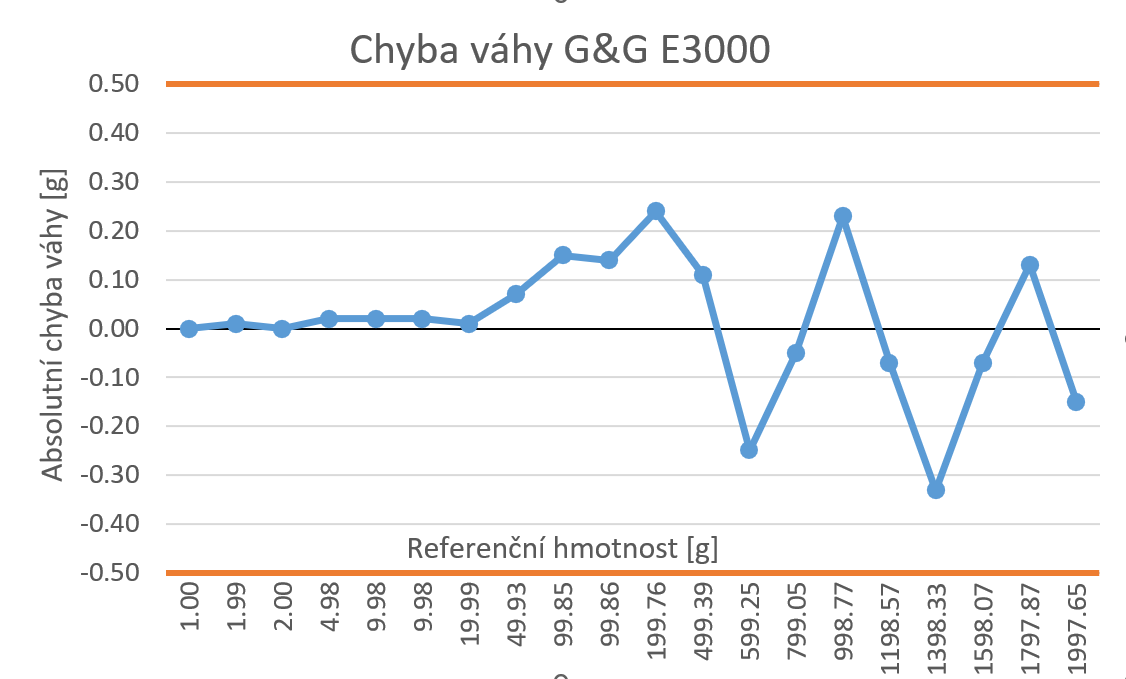
\includegraphics[scale=0.7]{obrazky/mereni.PNG}
    \end{center}
    \caption{Nalevo Kern PCB-2500-2, napravo G\&G E3000}
    \label{adapter}
\end{figure}

\begin{figure}[H]
    \begin{center}
        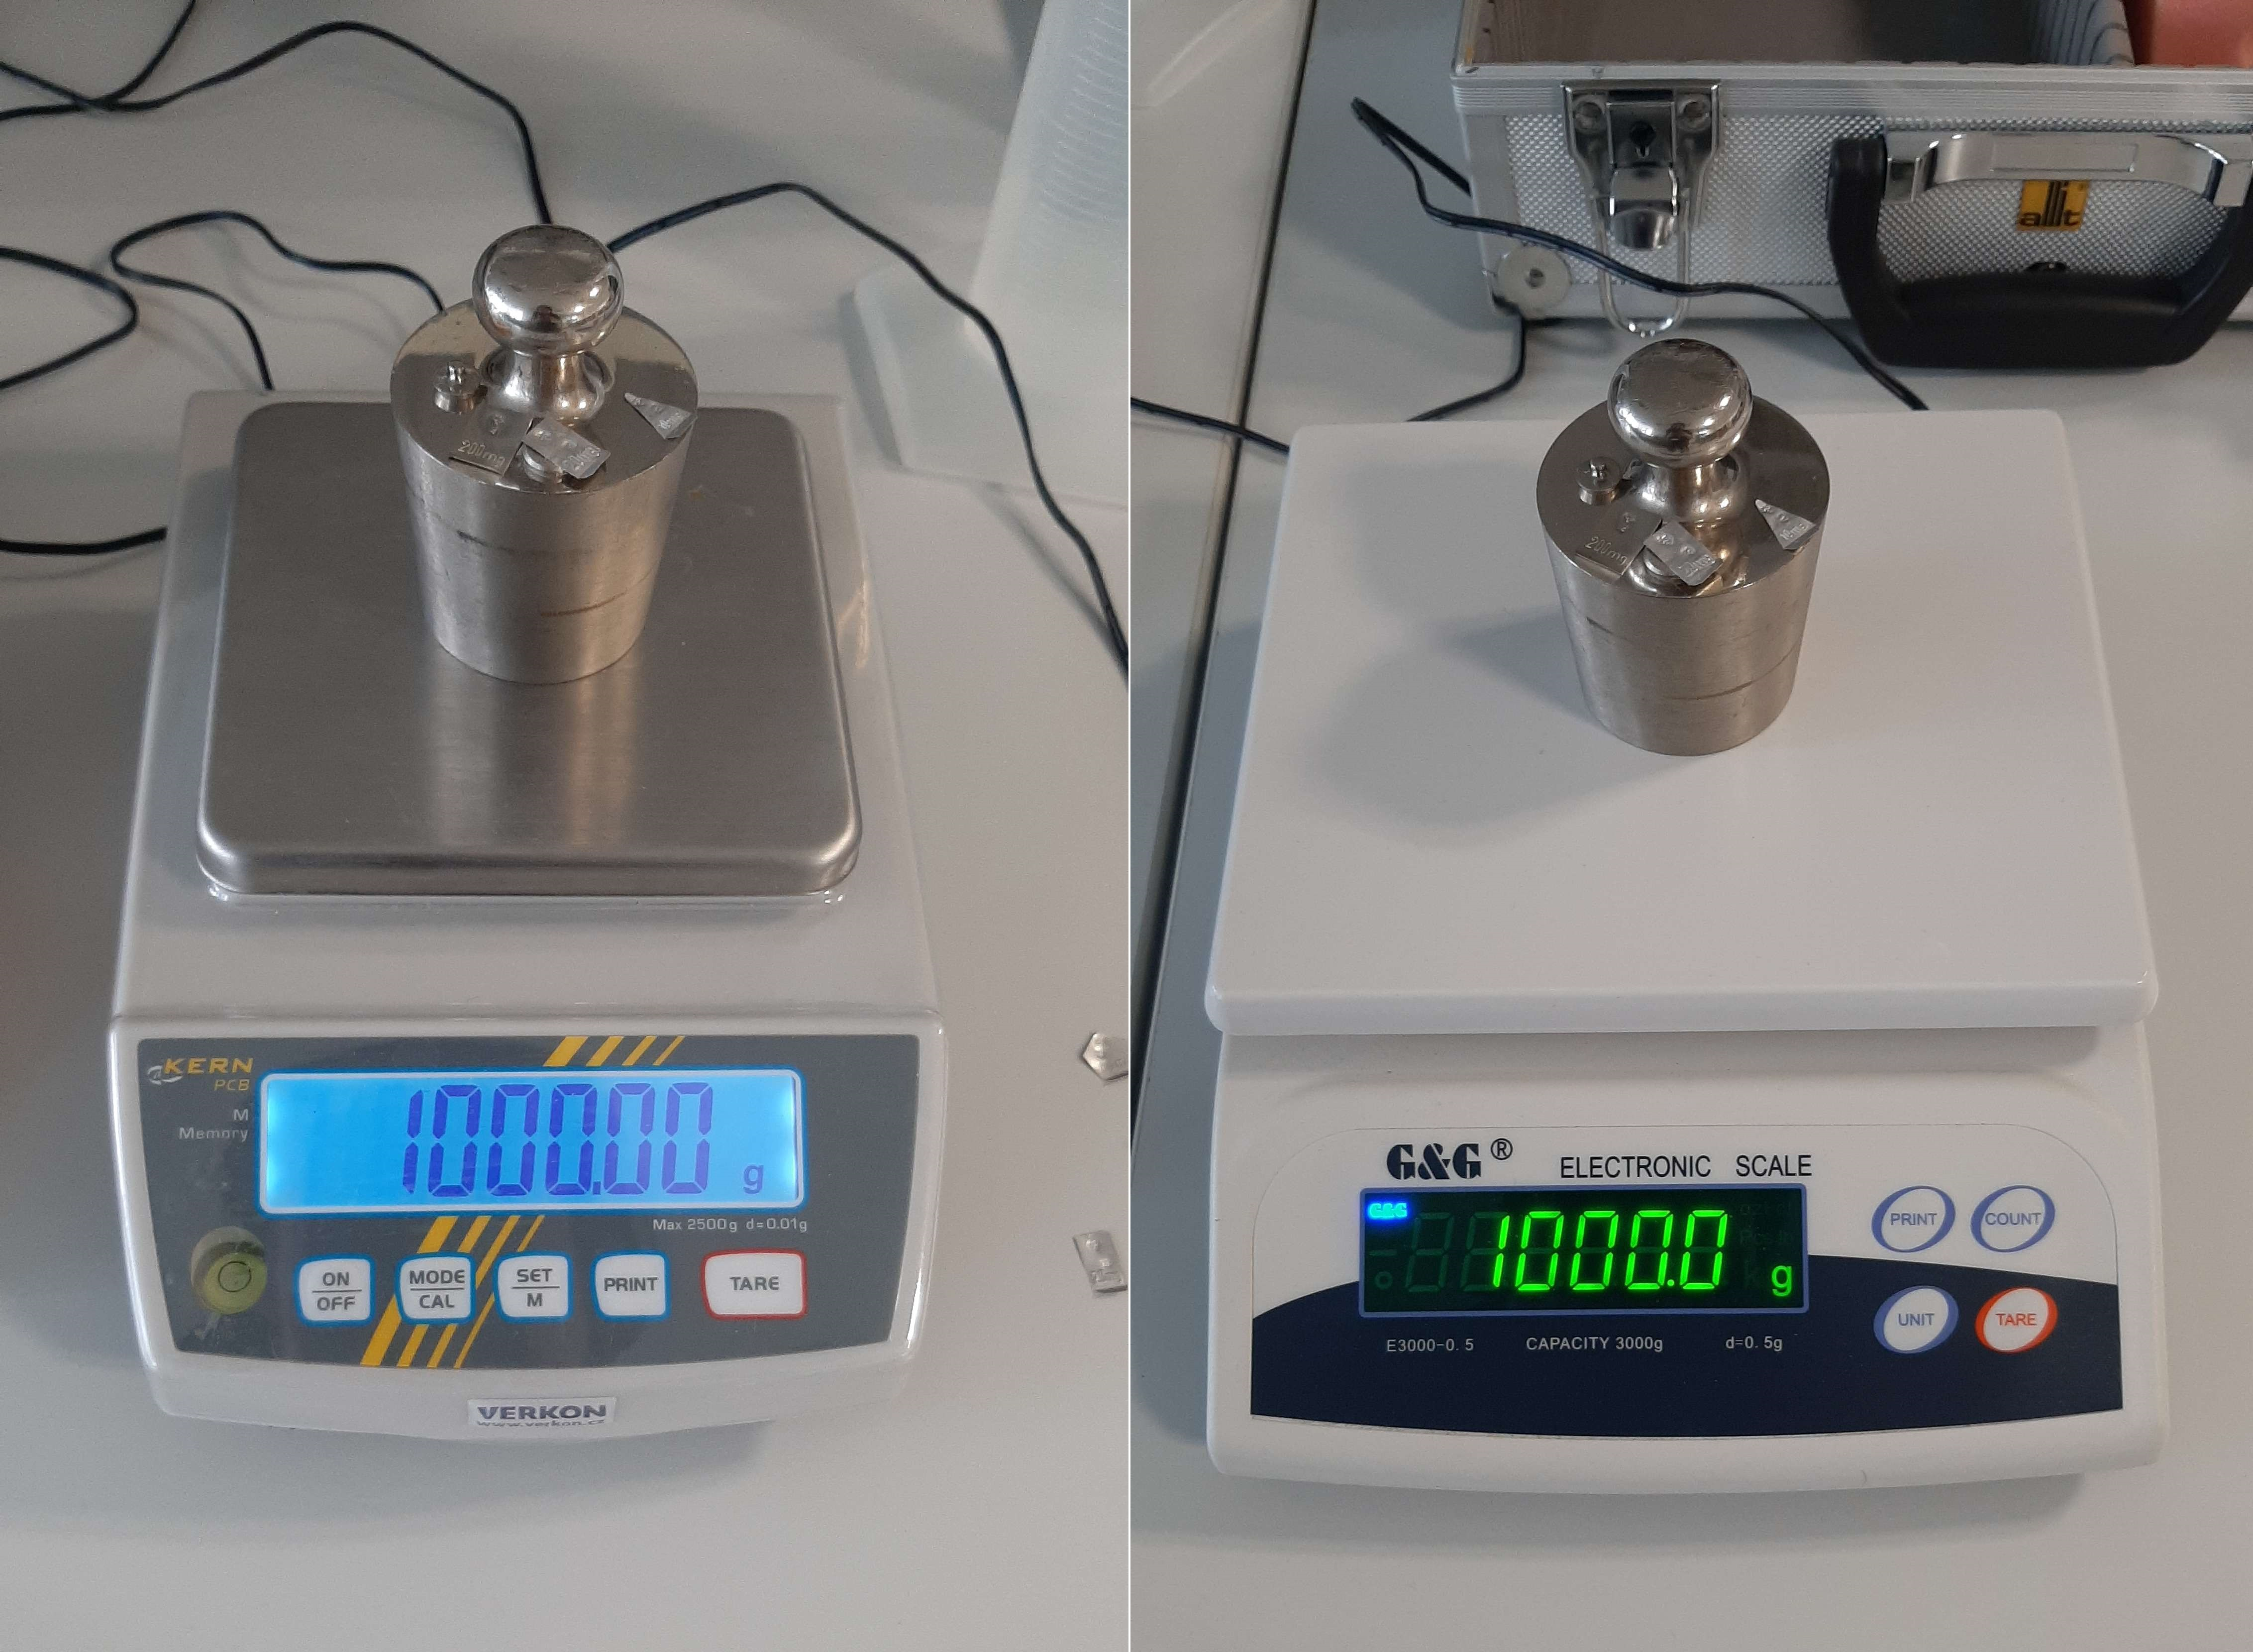
\includegraphics[scale=0.1]{obrazky/vahy.jpg}
    \end{center}
    \caption{Nalevo Kern PCB-2500-2, napravo G\&G E3000}
    \label{adapter}
\end{figure}

\section{Zprovoznění váhy}

Komunikační rozhraní váhy je RS-232, který nejsme schopni připojit na mikrokontrolér z důvodu absence totožného rozhraní. V takovém případě použijeme adaptér z RS-232 na USB. Použitý adaptér je ADS-50 USB - serial, který je součástí balení váhy. (obrázek č.\ref{adapter})

\begin{figure}[H]
    \begin{center}
        \includegraphics[scale=0.06]{obrazky/ADS-50 USB - serial adapter.png}
    \end{center}
    \caption{Adaptér USB - serial AXAGO ADS-50}
    \label{adapter}
\end{figure}

Propojení kabelu ADS-50 s váhou není možné z důvodu, že kabel není křížený, jinak zvaný "null modem" kabel. To znamená, že vysílací piny(Tx) jsou navzájem propojené a to samé přijímací piny(Rx). Aby komunikace mohla fungovat je nutné propojit Tx s Rx. Tato podmínka komunikace je zmíněná v dokumentaci váhy[x]. Výrobce váhy z tohoto důvodu k balení přidal kříženou redukci DB9(samice) - DB9(samice), která slouží současně k monitorování stavu jednotlivých pinů díky přídavným konektorům pro připojení např. osciloskopu. Dále výrobce přidal redukci DB9(samec) - DB9(samec) pro propojení křížené redukce s váhou(samice). Zapojení je možné vidět na obrázku č.\ref{propojení váhy v1}. Toto zapojení není praktické pokud nechceme diagnostikovat komunikaci, proto je možností koupit přímo křížený kabel nebo kříženou redukci, která vychází 5x levněji. Na obrázku č.\ref{propojení váhy v2} je výsledné řešení propojení váhy s mikrokontrolerem pomocí křížené redukce DB9(samec) - DB9(samice).

\begin{figure}[H]
    \begin{center}
        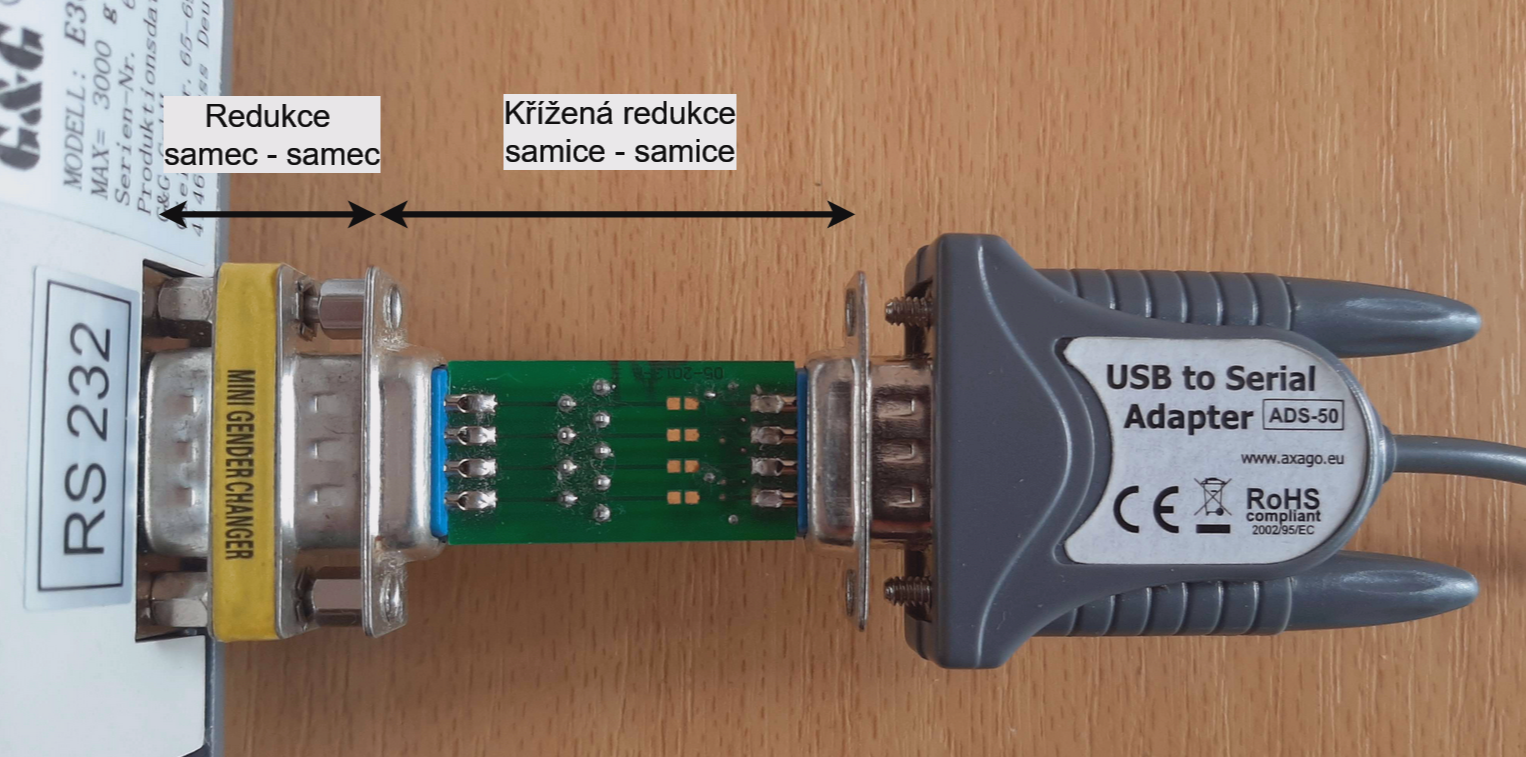
\includegraphics[scale=0.27]{obrazky/zapojeni_vahy_v1 - popis.png}
    \end{center}
    \caption{Propojení váhy s mikrokontrolerem pomocí komponent dodané výrobcem váhy}
    \label{propojení váhy v1}
\end{figure}

\begin{figure}[H]
    \begin{center}
        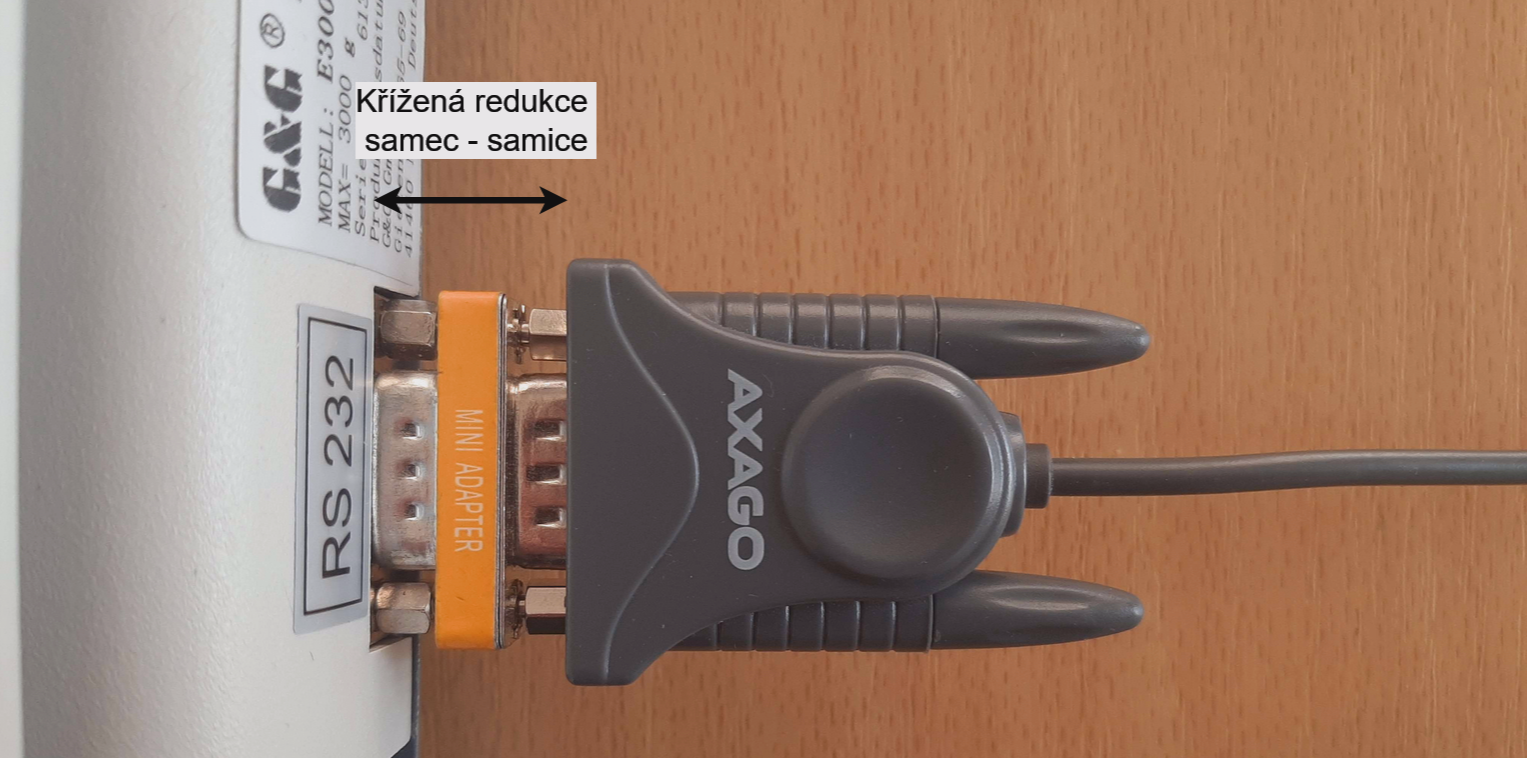
\includegraphics[scale=0.27]{obrazky/zapojeni_vahy_v2 - popis.png}
    \end{center}
    \caption{Výsledné propojení váhy s mikrokontrolerem}
    \label{propojení váhy v2}
\end{figure}

Dalším krokem je nastavení parametrů sériové komunikace podle manuálu váhy\cite{vaha_datasheed}. Komunikace byla testována pomocí osciloskopu s funkcí čtení UART protokolu a windows nástroje PuTTY, který přijímal/odesílal data po sériové lince. 
Na obrázku č. \ref{putty} je nastavení parametrů v PuTTY a na obrázku č.\ref{puttyyyy} je vidět, že váha nám na výstup konzole PuTTY posílá aktuální naměřená data.


\begin{figure}[H]
    \begin{center}
        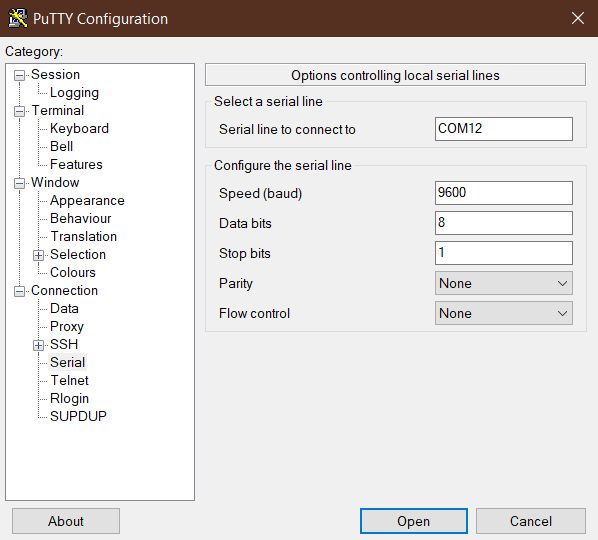
\includegraphics[scale=0.8]{obrazky/nastaveni putty.png}
    \end{center}
    \caption{Nastavení parametrů komunikace v PuTTY}
    \label{putty}
\end{figure}

\begin{figure}[H]
    \begin{center}
        \includegraphics[scale=0.09]{obrazky/komunikace váha putty.jpg}
    \end{center}
    \caption{Čtení sériové komunikace váhy pomocí PuTTY}
    \label{puttyyyy}
\end{figure}

Na obrázku č.\ref{osc} byl datový výstup váhy testován pomocí osciloskopu. Parametry na osciloskopu byly nastaveny obdobně jak na obrázku č.\ref{putty}

\begin{figure}[H]
    \begin{center}
        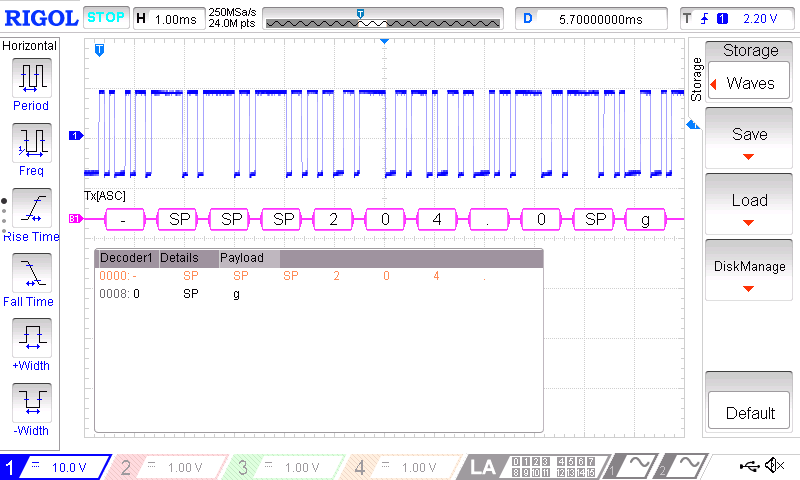
\includegraphics[scale=0.5]{obrazky/DS1Z_QuickPrint6.png}
    \end{center}
    \caption{Odchycení zprávy "-204.0 g" pomocí osciloskopu}
    \label{osc}
\end{figure}

%%%%%%%%%%%%%%%%%%%%%%%%%%%%%%%%%%%%%%%%%%%%%%%%%%%%%%%%%%%%%%%%%%%%%%%%%%%%%%%%%%%%%%%%%%%%%%%%%%%%%%%%%%%%%%%%%%%%%%%%%%%%%%%%
\section{Zprovoznění čtečky čárového kódu}
\label{zprovozeni_ctecky}
%Čtečka čárového kódu ve výchozím nastavení se chová jako klávesnice(HID KBW), aby bylo možné číst sériovou komunikaci je nutné naskenovat QR kód z manuálu\cite{scaner}, který přepíná výstup čtečky z HID KBW na virtuální sériový USB port(USB VCom).

Čtečka čárového kódu se ve výchozím nastavení chová jako klávesnice (USB HID KBW). To znamená, že pokud máme otevřený textový editor (například Word) a načteme čárový kód, data se vypíšou přímo do dokumentu, jako by byla zadána z běžné klávesnice.

Tento režim je však pro programové zpracování dat nepraktický – neumožňuje obousměrnou komunikaci, data nejsou strukturována do žádného rámce a není možné spolehlivě rozlišit začátek a konec zprávy. Výstup je navíc směrován do aktivního okna systému, což ztěžuje jeho přesné zachycení v aplikacích.

Z těchto důvodů výrobce poskytuje možnost přepnout čtečku do režimu USB VCOM (virtuální COM port). V tomto režimu čtečka emuluje sériový port přes USB, což umožňuje snadné a přesné čtení výstupu v programech jako je Python, HTerm nebo PuTTY – včetně možnosti odesílat příkazy zpět do čtečky.
\\\\
Čtečka tedy nabízí 3 komunikační rozhraní:
\begin{itemize}
    \item \textbf{UART} - Jeden z nejjednodušších sériových komunikačních protokolů, viz kapitola č. \ref{UART protokol}. Připojení k Raspberry Pi pomocí označených GPIO pinů: Tx a Rx. 
    \item \textbf{USB HID (Human Interface Device)}
    \begin{itemize}
        \item \textbf{USB HID KBW (Keyboard)} - emulace klávesnice (výchozí nastavení)
        \item \textbf{USB HID POS (Point of Sales)} - speciální protokol pro POS aplikace 
    \end{itemize}
    \item \textbf{USB VCom} - Virtuální sériový COM port, který emuluje UART komunikaci přes USB. Oproti klasickému UART rozhraní je USB VCOM stabilnější (integrovaná nízkoúrovňová CRC kontrola přenosu), jednodušší na zapojení a automaticky detekuje odpojení kabelu.
\end{itemize}
\bigskip
Po zapnutí se čtečka může nacházet ve třech různých provozních stavech, které jsou navrženy s ohledem na minimalizaci elektrické spotřeby:
\begin{itemize}
    \item \textbf{Operating (160 mA)} – Čtečka je aktivní a nachází se v režimu čtení. Je schopna okamžitě snímat a dekódovat čárové kódy.
    \item \textbf{Standby (30 mA)} – Čtečka se nachází v pohotovostním režimu, ve kterém čeká na aktivační impuls (např. detekce pohybu před senzorem, příkaz po sériové lince nebo stisk tlačítka). Po přijetí podnětu automaticky přechází do režimu čtení.
    \item \textbf{Sleep (3 mA)} – Nízkopříkonový režim, do kterého čtečka přechází po delší době nečinnosti. Funguje obdobně jako režim standby, avšak s výrazně nižší spotřebou energie. Nevýhodou je delší doba probuzení do režimu čtení (operating).
\end{itemize}
\bigskip
Čtečka čárového kódu má několik režimů čtení:
\begin{itemize}
    \item \textbf{Manuální (Manual)} - Pomocí fyzického tlačítka na těle čtečky.
    \item \textbf{Kontinuální (Continuous)} - Nepřetržité čtení.
    \item \textbf{Indukční (Induction)} - Čeká v standby režimu dokud nedetekuje změnu v obraze, pak se přepne do operating režimu.
    \item \textbf{Vyvolaný příkazem (Command Triggered)} - Čtečka začne skenovat po přijetí příkazu. Vhodné pro ovládání čtečku programem.
    \item \textbf{POS} - Přednastavený Command Triggered režim pro pokladní systémy - vypnutí oznamovacího zvuku při zapnutí čtečky, pakety posílány po sériové lince jsou bez ukončovacího znaku.
\end{itemize}
\bigskip
Funkčnost čtečky byla ověřena v režimu čtení \textit{Triggered} prostřednictvím rozhraní USB VCom za použití nástroje HTerm. Tento nástroj, na rozdíl od PuTTY, umožňuje odesílání dat ve formátu hexadecimálních řetězců, což je zásadní pro inicializaci čtečky do \textit{operating režimu} – stavu, ve kterém je schopna aktivně detekovat a dekódovat čárové kódy. Na základě technické dokumentace je pro spuštění skenovací sekvence nutné odeslat specifický příkaz ve formátu [\textbf{0x7E 0x00 0x08 0x01 0x00 0x02 0x01 0xAB 0xCD}], přičemž zařízení v případě úspěšného přijetí odpoví potvrzovací zprávou (tzv. ACK - \textit{acknowledgement code}) ve tvaru [\textbf{0x02 0x00 0x00 0x01 0x00 0x33 0x31}]. Výsledek této komunikace je zachycen na obrázku č. \ref{Zprovoznění čtečky}. Parametry pro sériovou komunikaci byly nastaveny stejně jak u váhy[\ref{putty}].

\section{Integrace čtečky do řídicí logiky systému}
% ME: Implementace čtečky do stavového automatu / Ovládání / Obsluha čtečky / Výběr čtecího režimu
% AI: Integrace čtečky do řídicí logiky systému / Řízení čtečky pomocí stavového automatu / Výběr čtecího režimu pro řízené snímání
Čtečka bude řízena programově prostřednictvím stavového automatu a aktivována pouze v okamžiku, kdy je potřeba provést identifikaci alkoholu (např. načtením EAN kódu nebo ručním výběrem produktu). Naskenování čárového kódu bude doprovázeno zvukovou a optickou signalizací – prostřednictvím integrované LED diody a bzučáku, které automaticky reagují při úspěšném přečtení kódu. LED dioda zároveň slouží k nasvícení kódu v podmínkách se zhoršenou viditelností.

V rámci návrhu stavového automatu je nutné čtečku z pohledu uživatele „zapínat“ (Operating režim) a „vypínat“ (Standby režim), aby nedocházelo k nechtěnému čtení a tím i chybné signalizaci nebo přenosu dat. V běžném provozu bohužel čtečku nelze explicitně přepnout příkazem do Standby režimu. Například v režimu Triggered přejde čtečka do Standby buď po úspěšném načtení kódu, nebo po uplynutí definovaného časového intervalu (0.1 – 25 s). Pokud však uživatel kód neoskenuje (např. zvolí produkt ručně), čtečka zůstane v aktivním režimu a je možné omylem načíst další kódy i mimo určený stav automatu.

Jelikož přechod mezi režimy nelze ovládat přímo příkazem, jedinou možností řízení ze strany programu bez nutnosti restartu čtečky zůstává zapínání/vypínání LED a bzučáku. Níže jsou uvedeny možné varianty, jak se s tímto omezením vyrovnat:

\begin{itemize}
    \item \textbf{Přerušení napájení} - Pomocí externího spínacího obvodu (např. tranzistoru řízeného přes GPIO), který by odpojil napájení čtečky nebo čtečku napájet přímo GPIO pinem, který by se spínal - Tento přístup by neumožňoval připojení přes USB a vyžadoval by komunikaci přes rozhraní UART.
    \item \textbf{Vymazání vstupního bufferu} - Čtečka sice nejde explicitně přepnout do Standby režimu, ale lze ji ponechat aktivní s vypnout LED a zvukovou signalizací. Z pohledu uživatele čtečka působí jako neaktivní, protože neposkytuje žádnou zpětnou vazbu, i když stále čte. Pokud dojde k náhodnému načtení kódu mimo požadovaný stav, příslušná data se uloží do vstupního bufferu mikrokontroléru, který lze následně programově vyprázdnit. Tento přístup lze využít například v režimu Continuous, kdy čtečka zůstává trvale aktivní.
    \item \textbf{Periodické spouštení čtečky} - V Triggered režimu nastavit krátký interval čtení a periodicky odesílat příkaz ke spuštění čtečky (Operating režim). Tato metoda není nejvhodnější z hlediska časové a výpočetní náročnosti – program je neustále přerušován odesíláním příkazů v krátkých intervalech a čekáním na ACK.
    \item \textbf{Přepínání do manuálního režimu} (aktuální řešení): V Manual režimu čtečka čeká v standby stavu dokud uživatel nezmáčkne tlačítko, tohle tlačítko ve finální verzi měřícího systému nebude fyzicky přístupné (čtečka bude schovaná v krabičce). Čtečka na základě stavového automatu bude přepínána mezi Countiual a Manual režimem.
\end{itemize}




\begin{figure}[h]
    \begin{center}
        \includegraphics[scale=0.14]{obrazky/Zprovoznění čtečky.png}
    \end{center}
    \caption{Čtení sériové komunikace čtečky pomocí HTerm}
    \label{Zprovoznění čtečky}
\end{figure}

%Čtečku bude spuštěna jen v určitém stavu programu, proto využijeme trigger mode, který nám zajístí, že uživatel nenačte čárový kod kdy nemá. To může způsobit hromadění kodu v bufferu mikrokontroleru/řídící jednotky
\\\\
%Čtečku čárového kódu lze připojit pomocí UART nebo USB rozhraní.

%Zjistit v jakem formatu mi to posílá

%%%%%%%%%%%%%%%%%%%%%%%%%%%%%%%%%%%%%%%%%%%%%%%%%%%%%%%%%%%%%%%%%%%%%%%%%%%%%%%%%%%%%%%%%%%%%%%%%%%%%%%%%%%%%%%%%%%%%%%%%%%%%%%%
\section{Zprovoznění dotykového displeje}
%Vybraný dotykový displej JOY-IT, má rozlišení 1024 x 600 px s poměrem stran 128:75, což přibližně odpovídá poměru 17:10. Raspberry Pi OS vybírá rozlišení podle seznamu podporovaných rozlišení CEA (Consumer Electronics Association) a DMT (Display Monitor Timings), které jsou standardní a široce kompatibilní s většinou monitorů a televizí. Rozlišení vybraného displeje nespadá do žádné zmíněné kategorie a je nutné jej nastavit ručně prostřednictvím systémového souboru 'config.txt' .[z1][z2] Pokud by rozlišení displeje se neshodovalo s rozlišením obrazovky, tak by se obraz musel škálovat (upraven tak, aby se vešel na fyzický rozměr displeje, což znamená jeho zvětšení nebo zmenšení), což by vedlo ke snížení kvality obrazu, dále pokud by rozlišení obrazovky překročilo rozlišení displeje, tak by došlo k většímu vytížení GPU.

Vybraný dotykový displej JOY-IT má rozlišení 1024×600 px a poměr stran 128:75, což přibližně odpovídá poměru 17:10. Systém Raspberry Pi OS automaticky volí rozlišení z nabídky standardizovaných režimů CEA (Consumer Electronics Association) a DMT (Display Monitor Timings), které jsou široce kompatibilní s většinou monitorů a televizorů. Rozlišení vybraného displeje nespadá do žádné zmíněné kategorie a je nutné jej nastavit ručně úpravou systémového souboru config.txt, konfiguračního souboru 10-monitor.conf. nebo využít utilit pro nastavení obrazu displeje, např. Xrandr.[z1][z2]
Pokud by se skutečné rozlišení displeje neshodovalo s nastaveným rozlišením obrazovky, byl by obraz škálován (zvětšen nebo zmenšen na fyzickou velikost displeje), což by zhoršilo jeho kvalitu. V případě, že by rozlišení obrazovky překročilo nativní rozlišení displeje, došlo by současně k větší zátěži GPU.

\subsection{Nastavení rozlišení obrazovky pomocí utility Xrandr}
%Použijem příkaz "cvt" (Coordinated Video Timing), který pro zvolené rozlišení vypíše informaci, jako je obnovovací frekvence, horizontální frekvence synchronizace (hsync) a pixel clock (pclk). Tyto informace jsou nutné pro nastavení nového rozlišení pomocí Xrandr.
%Pro nastavení nového rozlišení využívám příkaz "cvt" (Coordinated Video Timing), který poskytuje podrobné informace o zvoleném rozlišení, včetně obnovovací frekvence, horizontální frekvence synchronizace (hsync) a pixel clock (pclk). Tyto údaje jsou nezbytné pro konfiguraci nového rozlišení pomocí nástroje Xrandr.

Pro nastavení nového rozlišení (1024×600 px) využívám nástroj Xrandr, který vyžaduje znalost konkrétních časovacích parametrů – obnovovací frekvence, horizontální frekvence synchronizace (hsync) a pixel clocku (pclk). Tyto hodnoty získám z příkazu cvt (Coordinated Video Timing), který je dopočítá na základě požadovaného rozlišení.

%Pro konfiguraci nového rozlišení jsem  nového rozlišení využil jsem
%Pro konfiguraci rozlišení v linuxovém prostředí exituje více druhů nástrojů, já jsem si zvolil Xrandr, který vyžaduje výše zmíněné informace z příkazu "cvt"

%language = bash nebo sh
%%%%%%%%%%%%%%%%%%%%%%%%%%%%%%%%%%%%%%%%%%%%%%%%%%%%%%%%%%%%%%%%%
\captionsetup[lstlisting]{labelformat=empty}
\lstdefinelanguage{bashcolored}{
  language=bash,
  basicstyle=\ttfamily\small,
  commentstyle=\color{gray},
  keywordstyle=\color{blue},
  moredelim=**[is][\color{gray}]{@}{@}, % výstup obarvíš pomocí @...@
}
\begin{lstlisting}[language=bashcolored, caption=Příklad použití příkazu cvt (Linux terminál):, frame=single, breaklines=true, postbreak=\mbox{\textcolor{gray}{$\hookrightarrow$}\space}]
$cvt 1024 600
# 1024x600 59.85 Hz (CVT) hsync: 37.35 kHz; pclk: 49.00 MHzxa
@Modeline "1024x600\_60.00"   49.00  1024 1072 1168 ... [1]@

\end{lstlisting}
%\footnotemark
\footnotetext[1]{Plné znění odpovědi: \texttt{Modeline "1024x600\_60.00"   49.00  1024 1072 1168 1312  600 603 613 624 -hsync +vsync}}

\begin{lstlisting}[language=bash, caption=Na základě nově vygenerovaných parametrů vytvoříme nový režim pomocí Xrandr:, frame=single]
$xrandr --newmode  "1024x600\_60.00" 49.00 1024 ... [2]
\end{lstlisting}
\footnotetext[2]{Plné znění příkazu: \texttt{\$xrandr --newmode  "1024x600\_60.00"   49.00  1024 1072 1168 1312  600 603 613 624 -hsync +vsync}}

\begin{lstlisting}[language=bash, caption=Nově vytvořený režim přiřadíme k požadovanému video výstupu (např. HDMI-1):, frame=single]
$xrandr --addmode HDMI-1 "1024x600\_60.00"
\end{lstlisting}

\begin{lstlisting}[language=bash, caption=Nyní změníme rozlišení obrazovky:, frame=single]
$xrandr --output HDMI-1 --mode "1024x600\_60.00"
\end{lstlisting}
\captionsetup[lstlisting]{labelformat=default}
%%%%%%%%%%%%%%%%%%%%%%%%%%%%%%%%%%%%%%%%%%%%%%%%%%%%%%%%%%%







%%%%%%%%%%%%%%%%%%%%%%%%%%%%%%%%%%%%%%%%%%%%%%%%%%%%%%%%%%%%%
%Příklad použití příkazu cvt (terminál Linuxu):
%
%\$ cvt 1024 600
%
%\# 1024x600 59.85 Hz (CVT) hsync: 37.35 kHz; pclk: 49.00 MHzxa
%Modeline "1024x600\_60.00"   49.00  1024 1072 1168 1312  600 603 613 624 -hsync +vsync
%\\
%\\
%Následně vytvoříme nový režim pomocí Xrandr:
%
%\$xrandr --newmode  "1024x600\_60.00"   49.00  1024 1072 1168 1312  600 603 613 624 -hsync +vsync
%\\
%\\
%Nově vytvořený režim přidáme k požadovanému video výstupu (HDMI-1):
%
%\$xrandr --addmode HDMI-1 "1024x600\_60.00"
%\\
%\\
%Nyní změníme rozlišení obrazovky pomocí:
%
%\$xrandr --output HDMI-1 --mode "1024x600\_60.00"
%\\
%\\
%%%%%%%%%%%%%%%%%%%%%%%%%%%%%%%%%%%%%%%%%%%%%%%%%%%%%%%%%%%%%%
%Toto nastavení se neukládá a pokud chceme mít nově nastavené rozlišení i po opětovném spuštění raspberry pi je nutné jej uložit do souboru, který se spouští současně se systémem jako např. /etc/X11/xorg.conf.d/10-monitor.conf

%Toto nastavení není trvalé a aby zvolené rozlišení zůstalo zachováno i po opětovném spuštění Raspberry Pi, je třeba jej uložit do konfiguračního souboru, například \textbf{/etc/X11/xorg.conf.d/10-monitor.conf.}




%Nastavení rozlišení obrazovky pomocí systé

%V případě zvětšení(upscaling) by obraz ztrácel na přesnosti a byl by rozmazaný, zatím co při zmenšení(downscaling) by obraz ztrácel na detailech

%z1: raspbery dokumentace - co je v zadání BP
%z2: https://elinux.org/RPiconfig#Camera
